\documentclass[tikz,border=2pt]{standalone}
\usepackage{amsmath}
\usetikzlibrary{arrows.meta}
\begin{document}
% Job-market signalling game: Nature draws H (p = 0.4) or L (0.6); the worker (sender) sees her type
% and chooses e in {0,1}; the firm (receiver) sees e but not the type, so its two nodes after each e
% form one information set with belief mu(e) = P(H | e), and it pays w(e). Sender payoff w(e) - c_theta e,
% c_H = 0.5, c_L = 1.5.
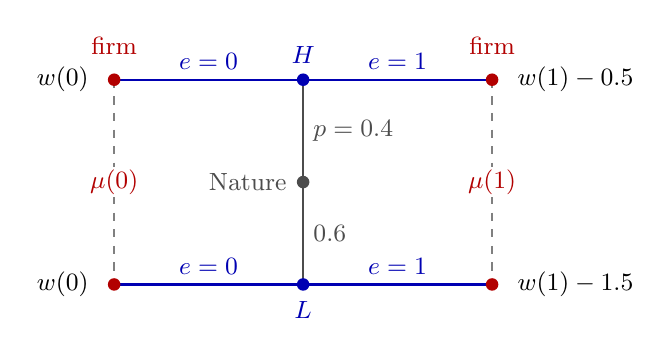
\begin{tikzpicture}[font=\small, >={Latex[length=2mm]},
    dec/.style={circle, fill, inner sep=1.6pt}]
  % Nature
  \draw[thick, gray!60!black] (0,0) -- node[right] {$p=0.4$} (0,1.3);
  \draw[thick, gray!60!black] (0,0) -- node[right] {$0.6$} (0,-1.3);
  \node[dec, gray!60!black, label={[gray!60!black]left:Nature}] at (0,0) {};
  % sender
  \foreach \y/\t in {1.3/H, -1.3/L} {
    \draw[thick, blue!70!black] (0,\y) -- node[above] {$e=0$} (-2.4,\y);
    \draw[thick, blue!70!black] (0,\y) -- node[above] {$e=1$} (2.4,\y);
  }
  \node[dec, blue!70!black, label={[blue!70!black]above:$H$}] at (0,1.3) {};
  \node[dec, blue!70!black, label={[blue!70!black]below:$L$}] at (0,-1.3) {};
  % receiver information sets
  \draw[thick, dashed, gray] (-2.4,1.3) -- (-2.4,-1.3);
  \draw[thick, dashed, gray] (2.4,1.3) -- (2.4,-1.3);
  \node[red!70!black, fill=white, inner sep=1pt] at (-2.4,0) {$\mu(0)$};
  \node[red!70!black, fill=white, inner sep=1pt] at (2.4,0) {$\mu(1)$};
  \foreach \x in {-2.4, 2.4} \foreach \y in {1.3,-1.3} \node[dec, red!70!black] at (\x,\y) {};
  \node[red!70!black, anchor=south] at (-2.4,1.5) {firm};
  \node[red!70!black, anchor=south] at (2.4,1.5) {firm};
  % sender payoffs after the wage w(e)
  \node[anchor=east] at (-2.6,1.3) {$w(0)$};
  \node[anchor=east] at (-2.6,-1.3) {$w(0)$};
  \node[anchor=west] at (2.6,1.3) {$w(1)-0.5$};
  \node[anchor=west] at (2.6,-1.3) {$w(1)-1.5$};
\end{tikzpicture}
\end{document}
